\documentclass[12pt,letterpaper]{article}
\usepackage[utf8]{inputenc}
\usepackage[spanish]{babel}
\usepackage{graphicx}
\usepackage[left=2cm,right=2cm,top=2cm,bottom=2cm]{geometry}
\usepackage{graphicx} % figuras
% \usepackage{subfigure} % subfiguras
\usepackage{float} % para usar [H]
\usepackage{amsmath}
%\usepackage{txfonts}
\usepackage{stackrel} 
\usepackage{multirow}
\usepackage{enumerate} % enumerados
\renewcommand{\labelitemi}{$-$}
\renewcommand{\labelitemii}{$\cdot$}
% \author{}
% \title{Caratula}
\begin{document}

% Fancy Header and Footer
% \usepackage{fancyhdr}
% \pagestyle{fancy}
% \cfoot{}
% \rfoot{\thepage}
%

% \usepackage[hidelinks]{hyperref} % CREA HYPERVINCULOS EN INDICE

% \author{}
\title{Caratula}

\begin{titlepage}
\begin{center}
\large{UNIVERSIDAD PRIVADA DE TACNA}\\
\vspace*{-0.025in}
\begin{figure}[htb]
\begin{center}

\includegraphics[width=4cm]{./Imagenes/logo}
\end{center}
\end{figure}
\vspace*{0.15in}
INGENIERIA DE SISTEMAS  \\

\vspace*{0.5in}
\begin{large}
TEMA:\\
\end{large}

\vspace*{0.1in}
\begin{Large}
\textbf{Informe Sesión de Laboratorio Nro 02 } \\
\end{Large}

\vspace*{0.3in}
\begin{Large}
\textbf{CURSO:} \\
\end{Large}

\vspace*{0.1in}
\begin{large}
BASE DE DATOS II\\
\end{large}

\vspace*{0.3in}
\begin{Large}
\textbf{DOCENTE(ING):} \\
\end{Large}

\vspace*{0.1in}
\begin{large}
 Patrick Jose Cuadros Quiroga\\
\end{large}

\vspace*{0.2in}
\vspace*{0.1in}
\begin{large}
Integrantes: \\
\begin{flushleft}

Marko Antonio RIVAS RIOS          	\hfill	(2016055461) \\
Jorge Luis MAMANI MAQUERA    	           \hfill	(2016055236) \\
Andree Ludwed VELASCO SUCAPUCA	\hfill	(2016055286) \\
Yofer Nain CATARI CABRERA		\hfill	(2017059289) \\
Adnner Sleyder ESPERILLA RUIZ		\hfill	(2015050543) \\
Jesus ESCALANTE ALANOCA           	\hfill	(2015050641) \\

\end{flushleft}
\end{large}
\end{center}

\end{titlepage}


\tableofcontents % INDICE
\thispagestyle{empty} % INDICE SIN NUMERO
\newpage
\setcounter{page}{1} % REINICIAR CONTADOR DE PAGINAS DESPUES DEL INDICE

\section{Ejercicio 1: Consultando Datos} 

\textbf{}\\
\textbf{}\\
Paso 1.Ingresar a Visual Studio y abrir o generar el proyecto que genera el contexto EF6-Code-First-Demo.

Paso 2. Agregar a la solución un Proyecto de pruebas unitarias .Net Framework.

\begin{center}
	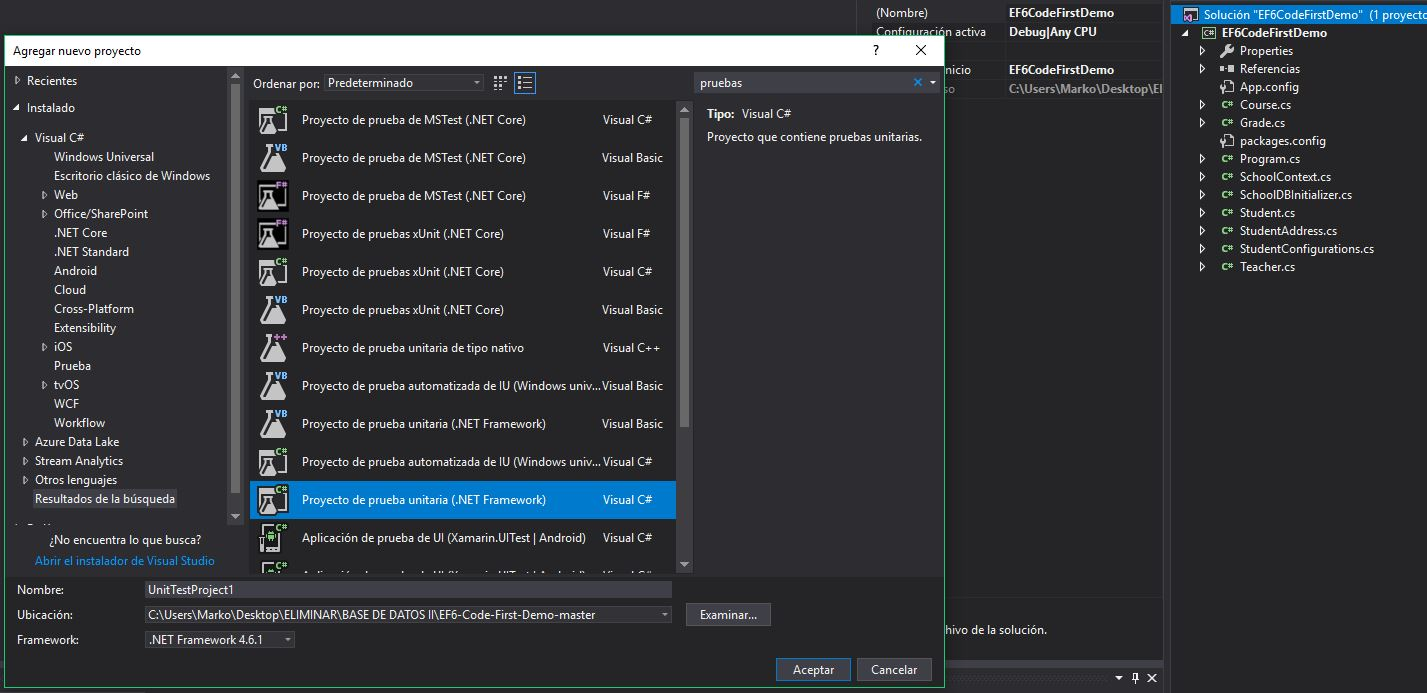
\includegraphics[width=10cm]{./Imagenes/Captura1} 
	\end{center}

Paso 3. En el proyecto de pruebas referenciar al proyecto principal al proyecto de pruebas

\begin{center}
	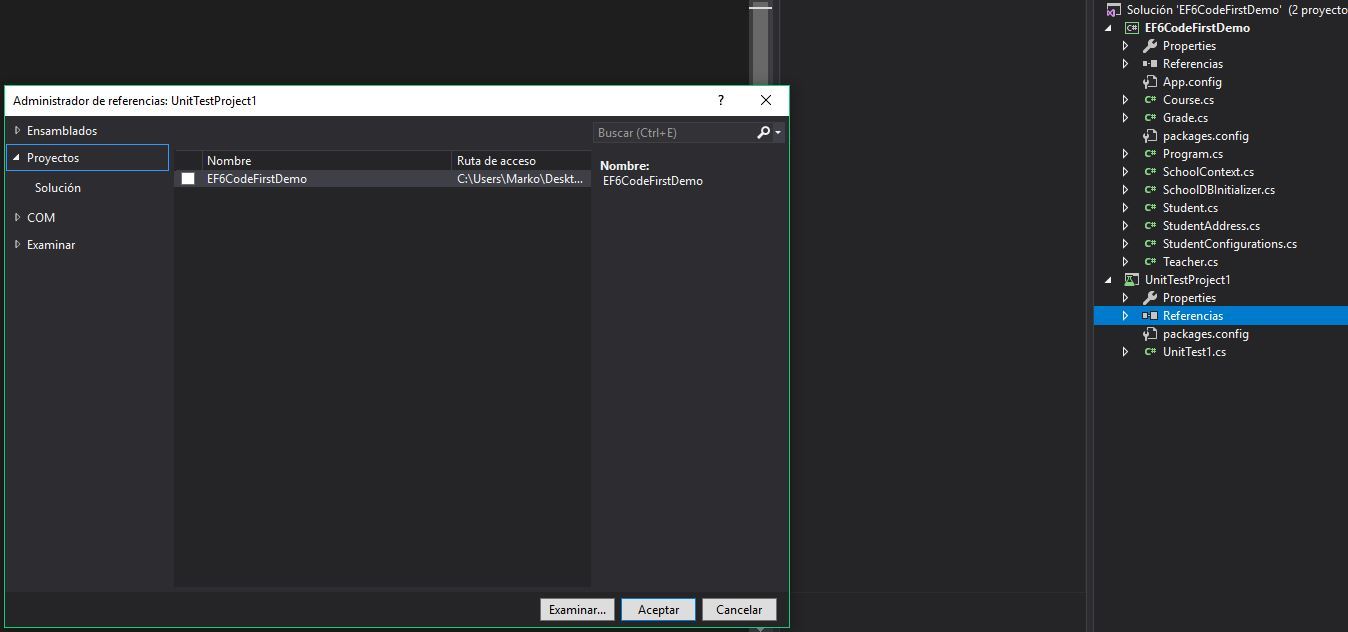
\includegraphics[width=10cm]{./Imagenes/Captura2} 
	\end{center}

Paso 4. En la clase Unitest generada crear el método: ObtenerAlEstudianteConIDUno, puede tomar como
referencia el siguiente código

\begin{center}
	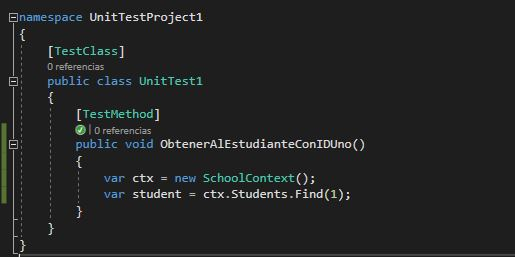
\includegraphics[width=10cm]{./Imagenes/Captura3} 
	\end{center}

\textbf{}\\
La sentencia SQL generada del lado del gestor de base de datos es: 

\begin{center}
	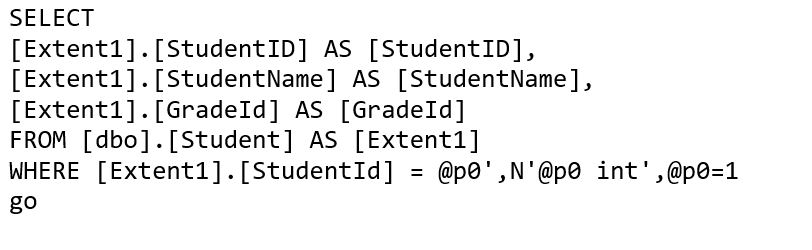
\includegraphics[width=10cm]{./Imagenes/U1-1} 
	\end{center}
\textbf{}\\

Paso 5. Adicionar otro método: BuscarAlPrimerEstudianteConElNombreBill, puede tomar como referencia el
siguiente código.

\begin{center}
	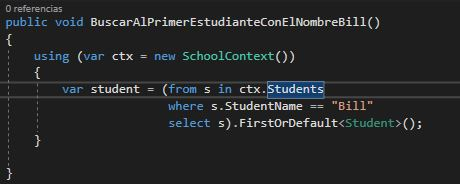
\includegraphics[width=10cm]{./Imagenes/Captura4} 
	\end{center}
\textbf{}\\

La sentencia SQL generada del lado del gestor de base de datos es: 

\begin{center}
	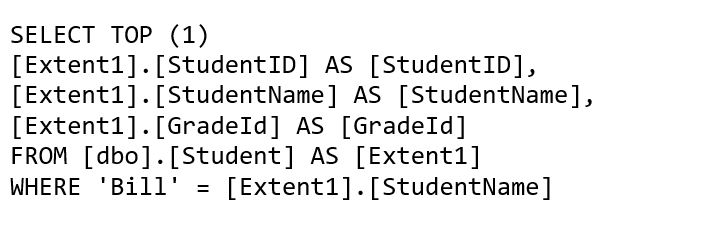
\includegraphics[width=10cm]{./Imagenes/U1-2} 
	\end{center}
\textbf{}\\
Paso 6. Agregar otro método de prueba denominado: BuscarEstudiantesAgrupadosPorGrado, tomar como
referencia el siguiente código.

\begin{center}
	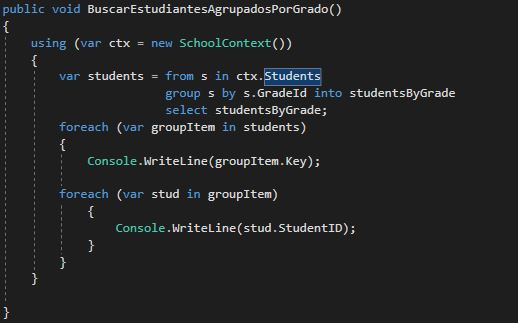
\includegraphics[width=10cm]{./Imagenes/Captura5} 
	\end{center}
\textbf{}\\

La sentencia SQL generada del lado del gestor de base de datos es: 


\textbf{}\\

Paso 7. Agregar otro método de prueba denominado: ObetenerListadoDeEstudiantesOrdenadosPorNombre, tomar
como referencia el siguiente código.

\begin{center}
	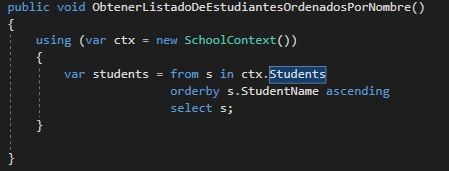
\includegraphics[width=10cm]{./Imagenes/Captura6} 
	\end{center}
\textbf{}\\

La sentencia SQL generada del lado del gestor de base de datos es: 

\begin{center}
	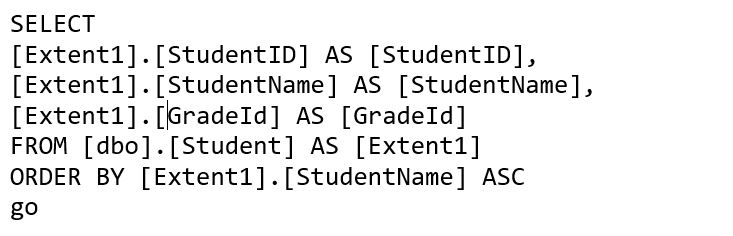
\includegraphics[width=10cm]{./Imagenes/U1-4} 
	\end{center}
\textbf{}\\

Paso 8. Finalmente crear el método de prueba: BuscarTodosLostudiantesConElEstandarUno, tomar como
referencia el siguiente código.

\begin{center}
	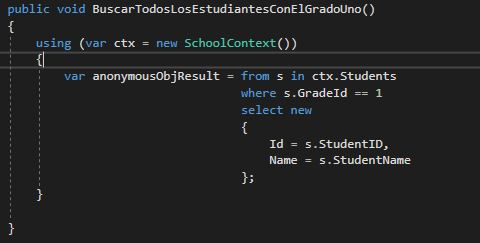
\includegraphics[width=10cm]{./Imagenes/Captura7} 
	\end{center}
\textbf{}\\

La sentencia SQL generada del lado del gestor de base de datos es: 

\begin{center}
	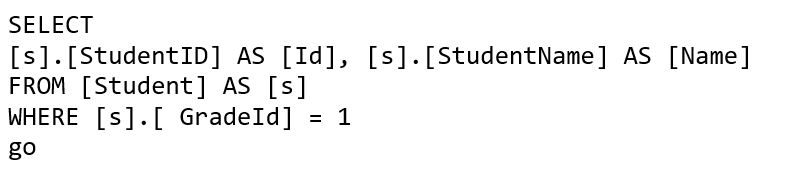
\includegraphics[width=10cm]{./Imagenes/U1-5} 
	\end{center}
\textbf{}\\
\textbf{}\\
\textbf{}\\

\section{Ejercicio 2: Guardando Datos} 

\textbf{}\\
\textbf{}\\
Paso 1. Agregar al proyecto de pruebas una clase de pruebas TestUnit02

\begin{center}
	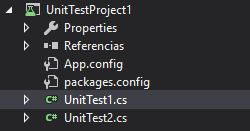
\includegraphics[width=10cm]{./Imagenes/Captura8} 
	\end{center}
\textbf{}\\

Paso 2. Agregar el método InsertarEstudianteSatisfactoriamente, tomar como referencia el siguiente código
\begin{center}
	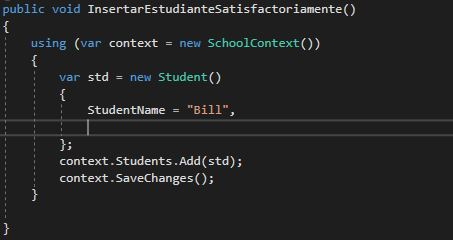
\includegraphics[width=10cm]{./Imagenes/Captura9} 
	\end{center}

\textbf{}\\
La sentencia SQL generada del lado del gestor de base de datos es:
\begin{center}
	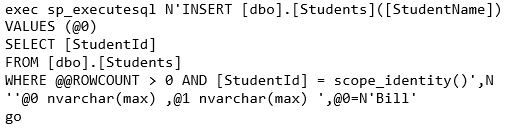
\includegraphics[width=10cm]{./Imagenes/U1-7} 
	\end{center}

\textbf{}\\
Paso 3. Agregar el método ActualizarAlPrimerEstudianteSatisfactoriamente, tomar como referencia el siguiente código
\begin{center}
	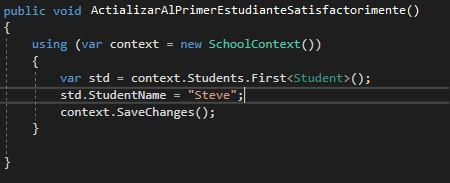
\includegraphics[width=10cm]{./Imagenes/Captura13} 
	\end{center}
\textbf{}\\
La sentencia SQL generada del lado del gestor de base de datos es:

\begin{center}
	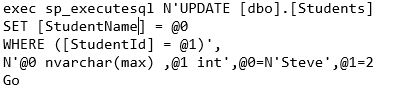
\includegraphics[width=10cm]{./Imagenes/U1-6} 
	\end{center}
\textbf{}\\
Paso 4. Agregar el método EliminarElPrimerEstudianteSatisfactoriamente, tomar como referencia el siguiente
código

\begin{center}
	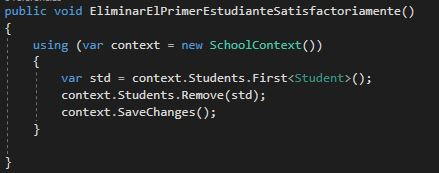
\includegraphics[width=10cm]{./Imagenes/Captura10} 
	\end{center}

\textbf{}\\
La sentencia SQL generada del lado del gestor de base de datos es:
\begin{center}
	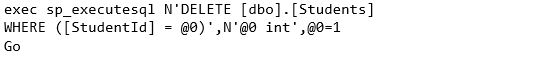
\includegraphics[width=10cm]{./Imagenes/U2-2} 
	\end{center}
\textbf{}\\
Paso 5. Agregar el método: AgregarTresEstudiantesSatisfactoriamente, tomar como referencia el siguiente código:

\begin{center}
	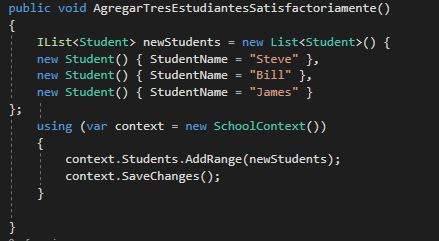
\includegraphics[width=10cm]{./Imagenes/Captura11} 
	\end{center}

\textbf{}\\
Paso 5. Finalmente agregar el método de pruebas: EliminarTresEstudiantesSatisfactoriamente, tomar como
referencia el siguiente código:

\begin{center}
	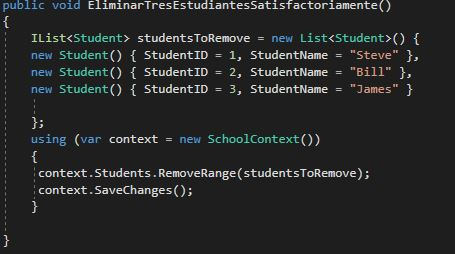
\includegraphics[width=10cm]{./Imagenes/Captura12} 
	\end{center}
\textbf{}\\







\end{document}